\documentclass[tikz,border=10pt]{standalone}
\usepackage{amsmath}
\usepackage{tikz}
\usetikzlibrary{arrows.meta, positioning, calc, shapes.geometric}

\begin{document}
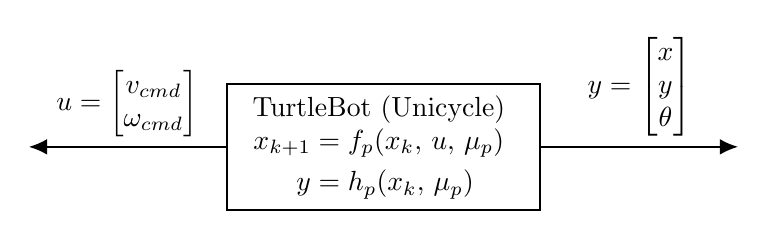
\begin{tikzpicture}[
  block/.style = {draw, thick, minimum height=3em, minimum width=6em, align=center},
  arrow/.style = {thick, -{Latex[width=2mm]}},
  node distance=2.5cm and 2.5cm
]

  % Plant
  \node[block] (plant) {
    \begin{tabular}{c}
      TurtleBot (Unicycle)\\
      $\begin{aligned}
      x_{k+1} &= f_p(x_k,\,u,\,\mu_p) \\
      y &= h_p(x_k,\,\mu_{p})
       \end{aligned}$
    \end{tabular}
  };

  % Input
  \draw[arrow] (plant.west) -- ++(-2.5,0) node[midway,above] {$u = \begin{bmatrix} v_{cmd} \\ \omega_{cmd} \end{bmatrix}$};

  % Output
  \draw[arrow] (plant.east) -- ++(2.5,0) node[midway,above] {$y = \begin{bmatrix} x \\ y \\ \theta \end{bmatrix}$};

\end{tikzpicture}
\end{document}
